\documentclass{beamer}

\usepackage[utf8]{inputenc}
\DeclareUnicodeCharacter{00A0}{ }%Permet d'éviter certains conflits de caractères invisibles
\usepackage{amssymb}            % Principaux symboles
%\usepackage{fontspec}
%\usepackage{xunicode}
%\usepackage{xltxtra}
\usepackage[frenchb]{babel}
%\defaultfontfeatures{Scale=MatchLowercase}
%\setmainfont[Mapping=tex-text,Ligatures={Common, Historical}]{Linux Libertine O}
%\setsansfont[Mapping=tex-text]{Linux Biolinum O}
%\setmonofont[Scale=0.75]{DejaVu Sans Mono}

%% Packages pour le texte
%\usepackage[misc,geometry]{ifsym}	% Police numéros battons
\usepackage{pifont}		% Police \ding
\usepackage{eurosym}		% Symbole de l'euro
\usepackage{soul}		% Souligner
\usepackage{enumerate}		% Listes
\usepackage{verbatim}		% Codes source
\usepackage{moreverb}		%	et listings
\usepackage{textcomp}
\usepackage{multicol}

%% Packages pour les tableaux
\usepackage{array}		% Outils supplémentaires
\usepackage{multirow}		% Colonnes multiples
\usepackage{tabularx}		% Largeur totale donnée
\usepackage{longtable}		% Sur plusieurs pages

%% Les packages pour les dessins
\usepackage{graphicx}		% Insertion de figures
%\usepackage{picins}		% Dans un paragraphe
\usepackage{epic}		% Capacités graphiques
\usepackage{eepic}		% 	étendues
\usepackage{afterpage}		% Voir page 69
\usepackage{rotating}		% Tourner du texte
\usepackage{caption}		% Légendes
% \addto\captionsfrench{\def\figurename{}}

%% Packages pour les maths
\usepackage{amsmath}		% Commandes essentielles
\usepackage{amssymb}		% Principaux symboles
\usepackage{mathrsfs}		% Police calligraphique
\usepackage{theorem}		% Théorèmes
%\usepackage{tikz}		% Courbes
\usepackage{esvect}            % Vecteurs
%\usetikzlibrary{shapes,arrows,shadows}
\usepackage{pgf}
%\usetikzlibrary{arrows}
% Packages pour la physique
%\usepackage{sistyle}		% Unités
\usepackage[version=3]{mhchem}	% Formules chimiques
\usepackage{etex}
%\usepackage{m-pictex,m-ch-en}

%\usepackage{media9}
\usepackage{multimedia}		% Vidéos dans la présentation
%\usepackage{movie15}

%Ajout d'images de fond:
\usepackage{eso-pic}
\usepackage{wallpaper}

\usepackage{ccicons}		% Licence creativecommons
\usepackage{xcolor,colortbl}

%\SIdecimalsign{,}


\AtBeginSection[]
{
  \begin{frame}
    \frametitle{Sommaire}
    \begin{multicols}{2}
      {\small
				\setcounter{tocdepth}{2}
        \tableofcontents[currentsection, hideothersubsections]}
    \end{multicols}
  \end{frame}
}

\usetheme{Warsaw}

\usepackage{tikz}
\usetikzlibrary{arrows,automata}
\usepackage{fancyvrb}
\usepackage[french,onelanguage]{algorithm2e}
\usepackage{hyperref}
\usepackage{tabularx}
\usepackage{makecell}
\usepackage{dirtytalk}
\usepackage{verbatim}
\usepackage{multicol}
\usepackage{xcolor}
\usepackage{color}
\definecolor{forestgreen}{rgb}{0.0, 0.27, 0.13}
\definecolor{frenchblue}{rgb}{0.0, 0.45, 0.73}

\useoutertheme{infolines}
\setbeamersize{text margin left=1cm,text margin right=1cm}

\title{Projet Web Pain Chocolatine}
\subtitle{INFO 305}
\author{Clerc Gregory, Wagner Robin, Pleinet Estelle, Porteries Tristan}

\begin{document}

\begin{frame}
  \titlepage
\end{frame}

\begin{frame}
    \frametitle{Sommaire}
    \begin{multicols}{2}
      {
% 		\setcounter{tocdepth}{1}
        \tableofcontents
      }
    \end{multicols}
\end{frame}

\section{Presentation du projet}

\subsection{Idée}

\begin{frame}{But du projet}
	Faciliter la gestion des commandes de petits commerces de vente. Par exemple des boulangeries.\\
	Prévision de la demande du jour par l'utilisation de réservation.
	\begin{center}
		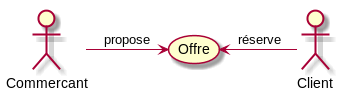
\includegraphics[width=10cm]{site_use.png}
	\end{center}
\end{frame}

\begin{frame}
	Les commerces proposent des produits puis des offres associèes~: l'horaire ou le produit peut être fabriqué et vendu.
	Les client liste les produits d'un commerce, puis ses offres et reserve une quantité de l'offre.
	\bigbreak
	Limitation de reservation~: quantité maximale totale, quantité maximale par client.
\end{frame}


\subsection{Exemple}

\begin{frame}{Le sandwich de Michel}
	\begin{center}
		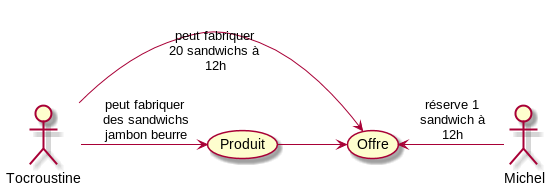
\includegraphics[width=10cm]{site_exemple.png}
	\end{center}
\end{frame}

\subsection{Cahier des charges}

\begin{frame}{Entités du système}
	Plusieurs entités sont nécessaire au fonctionnement du système.
	\begin{itemize}
		\item client (nom, mot de passe, email...)~;
		\item commerce (nom, mot de passe, email, adresse, produits...)~;
		\item produit (nom, prix, offres...)~;
		\item offre (quantité totale, quantité par personne)~;
		\item reservation (quantité).
	\end{itemize}

\end{frame}


\begin{frame}
	Liste des fonctionnalités défini avant l'écriture du site. \\
	fonctionnalités communes~;
	\begin{itemize}
		\item s'inscrire~;
		\item se connecter~;
		\item lister les commerces, offre, produit.
	\end{itemize}

	En tant que client~:
	\begin{itemize}
		\item reserver une offre~;
		\item lister ses réservations.
	\end{itemize}
	
	En tant que commerce~:
	\begin{itemize}
		\item ajouter un produit~;
		\item ajouter une offre~;
		\item lister ses clients (réservations)~;
		\item valider une reservation (le client la récupéré).
	\end{itemize}
\end{frame}

\section{Réalisation}

\subsection{Organisation de donnée}

\begin{frame}{Diagramme UML}
	\begin{center}
		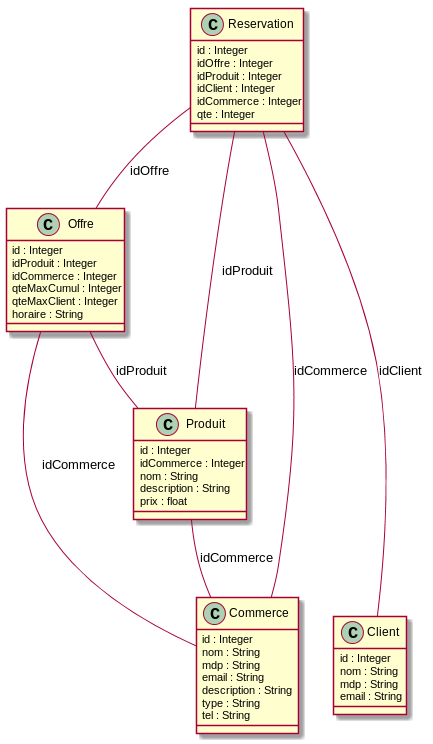
\includegraphics[height=8cm]{uml.png}
	\end{center}
\end{frame}

\begin{frame}
	Définition de classes PHP correspondant à chaque entité.
	\bigbreak
	Définition d'une table pour chaque classe avec les champs identiques à ceux des classes.
	\bigbreak
	Automatiser les fonctions de lecture et d'écriture de la base de donnée.
\end{frame}

\subsection{Analyse des fonctionnalités}

\begin{frame}
	Pour chaque classe, definition de fonctions pour~:
	\begin{itemize}
		\item ajouter~;
		\item récuperer par l'id~;
		\item lister par un identifiant~: par exemple lister les offres d'un produit~;
		\item supprimmer.
	\end{itemize}

	Définition dans include/ dans un fichier séparé par nom de classe.

\end{frame}

\subsection{Architecture du site}

\begin{frame}[fragile]
	\begin{multicols}{3}
		\tiny{
\color{blue}
		\begin{Verbatim}
css
  style.css
		\end{Verbatim}
\color{blue}
		\begin{Verbatim}
include
		\end{Verbatim}
\color{violet}
		\begin{Verbatim}
  db
    client.php
    commerce.php
    db.php
    image.php
    main.php
    offre.php
    produit.php
    reservation.php
    session.php
    statistique.php
    utilisateur.php
		\end{Verbatim}
\color{blue}
		\begin{Verbatim}
  error.php
  footer.php
  form.php
  header.php
  url.php
		\end{Verbatim}
\color{red}
		\begin{Verbatim}
index.php
		\end{Verbatim}
\color{black}
		\begin{Verbatim}
interface
		\end{Verbatim}
\color{red}
		\begin{Verbatim}
  action.php
		\end{Verbatim}
\color{blue}
		\begin{Verbatim}
  client
		\end{Verbatim}
\color{forestgreen}
		\begin{Verbatim}
    action
      connexion.php
      inscription.php
      reservation.php
      suppressionCompte.php
    		\end{Verbatim}
\color{frenchblue}
		\begin{Verbatim}
    ajouterReservation.php
    listerReservation.php
    listerStatistique.php
		\end{Verbatim}
\color{blue}
		\begin{Verbatim}
  commerce
		\end{Verbatim}
\color{forestgreen}
		\begin{Verbatim}
    action
      ajouterOffre.php
      ajouterProduit.php
      connexion.php
      inscription.php
      suppressionCompte.php
      supprimerOffre.php
      supprimerProduit.php
      validerReservation.php
    		\end{Verbatim}
\color{frenchblue}
		\begin{Verbatim}
    ajouterOffre.php
    ajouterProduit.php
    listerClients.php
    listerProduits.php
    listerStatistique.php
  		\end{Verbatim}
\color{blue}
		\begin{Verbatim}
  commun
    		\end{Verbatim}
\color{forestgreen}
		\begin{Verbatim}
    action
      commerce.php
      connexion.php
      deconnexion.php
      inscription.php
      offre.php
      produit.php
    		\end{Verbatim}
\color{frenchblue}
		\begin{Verbatim}
    connexion.php
    deconnexion.php
    gestionCompte.php
    inscription.php
    listerCommerces.php
    listerOffres.php
    listerProduits.php
		\end{Verbatim}
\color{blue}
		\begin{Verbatim}
uploads
		\end{Verbatim}
		}
	\end{multicols}
\end{frame}

\section{Répartition du travail et méthodes}

\subsection{Repartition}

\begin{frame}{Sous projets}
	3 sous projets~:
	\begin{itemize}
		\item interface base de donnée~;
		\item affichage et formulaire~;
		\item habillage CSS.
	\end{itemize}
\end{frame}

\begin{frame}{Partage du travail par équipe}
	2 équipes~:
	\begin{itemize}
		\item Robin, Greg~: CSS, affichage~;
		\item Estelle, Tristan~: formulaire, interface base de donnée.
	\end{itemize}

\end{frame}

\subsection{Gestion de version}

\begin{frame}{Git}
	Test en continue de la validité du travail de chaque personne.
\end{frame}

\subsection{Objectifs hebdomadaires}

\begin{frame}
	\begin{itemize}
		\item $1^{ere}$ semaine~;
		\item $2^{eme}$ semaine~;
		\item $3^{eme}$ semaine~;
		\item $4^{eme}$ semaine~;
		\item $5^{eme}$ semaine~;
	\end{itemize}

\end{frame}

\section{Démonstration}

\subsection{Exemple de la démonstration}

\end{document}
